
%% bare_conf.tex
%% V1.4b
%% 2015/08/26
%% by Michael Shell
%% See:
%% http://www.michaelshell.org/
%% for current contact information.
%%
%% This is a skeleton file demonstrating the use of IEEEtran.cls
%% (requires IEEEtran.cls version 1.8b or later) with an IEEE
%% conference paper.
%%
%% Support sites:
%% http://www.michaelshell.org/tex/ieeetran/
%% http://www.ctan.org/pkg/ieeetran
%% and
%% http://www.ieee.org/
%%*************************************************************************
%% Legal Notice:
%% This code is offered as-is without any warranty either expressed or
%% implied; without even the implied warranty of MERCHANTABILITY or
%% FITNESS FOR A PARTICULAR PURPOSE!
%% User assumes all risk.
%% In no event shall the IEEE or any contributor to this code be liable for
%% any damages or losses, including, but not limited to, incidental,
%% consequential, or any other damages, resulting from the use or misuse
%% of any information contained here.
%%
%% All comments are the opinions of their respective authors and are not
%% necessarily endorsed by the IEEE.
%%
%% This work is distributed under the LaTeX Project Public License (LPPL)
%% ( http://www.latex-project.org/ ) version 1.3, and may be freely used,
%% distributed and modified. A copy of the LPPL, version 1.3, is included
%% in the base LaTeX documentation of all distributions of LaTeX released
%% 2003/12/01 or later.
%% Retain all contribution notices and credits.
%% ** Modified files should be clearly indicated as such, including  **
%% ** renaming them and changing author support contact information. **
%%*************************************************************************



\documentclass[a4paper,conference]{IEEEtran}

\def\citepunt{,}

\usepackage[pdftex]{graphicx}
\ifCLASSOPTIONcompsoc
  \usepackage[caption=false,font=normalsize,labelfont=sf,textfont=sf]{subfig}
\else
  \usepackage[caption=false,font=footnotesize]{subfig}
\fi
\usepackage{comment}
\usepackage{float}
\usepackage{mathtools}
\usepackage{amsfonts}
\usepackage{bm}
\usepackage{siunitx}
\usepackage{pgf,tikz,pgfplots}
\usetikzlibrary{calc}

\DeclarePairedDelimiter\ceil{\lceil}{\rceil}
\DeclarePairedDelimiter\floor{\lfloor}{\rfloor}

\DeclareMathOperator{\vect}{vec}

\newcommand{\R}{\mathbb{R}}
\newcommand{\A}{\mathcal{A}}
\newcommand{\D}{\mathcal{D}}
\newcommand{\I}{\hat{I}}
\newcommand{\Z}{\mathbb{Z}}
\newcommand{\m}[1]{{\mathrm{\bf #1}}}
\newcommand{\E}{\tilde{\m{I}}}
\newcommand{\F}{\hat{F}}
\newcommand{\lI}{\m{I}}
\newcommand{\mF}{\m{F}}
\newcommand{\bF}{\mathcal{F}}
\newcommand{\J}{\hat{J}}
\newcommand{\lJ}{\m{J}}
\newcommand{\pD}{D^\prime}
\newcommand{\eF}{\hat{\mF}}
\newcommand{\gN}{\m{N}}
\newcommand{\W}{\m{W}}
\newcommand{\M}{\mathcal{M}}
\newcommand{\Pa}{\mathcal{P}}
\newcommand{\pDD}{\D^\prime}

\definecolor{navy}{RGB}{0,0,137}
\definecolor{tealDeer}{RGB}{148,232,180}
\definecolor{dodgerBlue}{RGB}{18,161,255}
\definecolor{citrine}{RGB}{230, 194, 8}
\definecolor{violet}{RGB}{112,5,164}
\definecolor{navyPurple}{RGB}{172,86,253}
\definecolor{heliotrope}{RGB}{236,93,253}

% correct bad hyphenation here
\hyphenation{op-tical net-works semi-conduc-tor}


\begin{document}

\title{Learning CNN filters from user-drawn image makers for coconut-tree image classification}

% make the title area
\maketitle

\begin{abstract}
Identifying species of trees in aerial images is essential for land-use classification, plantation monitoring, and impact assessment of natural disasters. The manual identification of trees in aerial images is tedious, costly, and error-prone, so automatic classification methods are necessary. Convolutional Neural Network (CNN) models have well succeeded in image classification applications from different domains. However, CNN models usually require intensive manual annotation to create large training sets. One may conceptually divide a CNN into convolutional layers for feature extraction and fully connected layers for feature space reduction and classification. We present a method that needs a minimal set of user-selected images to train the CNN's feature extractor, reducing the number of required images to train the fully connected layers. The method learns the filters of each convolutional layer from user-drawn markers in image regions that discriminate classes, allowing better user control and understanding of the training process. It does not rely on optimization based on backpropagation, and we demonstrate its advantages on the binary classification of coconut-tree images against one of the most popular CNN models.
\end{abstract}

\section{Introduction}
Deep learning has proven to be applicable to different tasks, from image classification to data synthesis \cite{goodfellow2016deep}. In remote sensing, the applications may involve segmentation of terrain images \cite{kemker2018algorithms, kampffmeyer2016semantic, hamaguchi2018effective}, building identification \cite{xu2018building, lu2018detecting, liu2018multilevel}, and deforestation monitoring \cite{bragilevsky2017deep}, for instance. In this work, we are interested in identifying species of trees from aerial images. The topic is important for land-use classification, plantation monitoring, and damage assessment of natural disasters. As the plantations can span vast areas, the manual identification of each tree is costly, tedious, and error-prone, and so automatic classification methods are necessary. 

Classification of tree species in aerial images has been actively investigated~\cite{fassnacht2016review}. In \cite{puttemans2018comparing} and~\cite{aparna2018cnn}, the authors present automatic solutions to detect coconut trees based on convolutional neural network (CNN) models. Despite these recent advances, CNN models usually require considerable human effort in image annotation to create large training sets. Vargas-Muñoz et al.~\cite{8899005} propose an active learning approach to mitigate the problem. The method explores data projection techniques to allow simultaneous annotation of multiple patches as having or not coconut trees. It then uses a CNN to identify the candidate patches with coconut trees. We adopt another alternative -- the design of simplified CNN models from small training sets with user interaction, being the user an expert in the design of CNN models. 


The design of CNN models without a human as part of the training loop leaves several questions unanswered: (1) How to find a useful and simplified model for a given classification problem? (2) How to train that model from a minimum number of annotated images?  (3) Can the user explain the decisions of the model? (4) Can the model improve from label corrections? The first question requires human knowledge about CNN modeling and the problem of interest. The second one requires to reduce the human effort to train a CNN model. The third issue is related to human understanding. It may explore data visualization techniques to explain the model's decisions and to guide the user in the design of the model. The fourth question is also essential during training, and it is related to user control over the process. They all lead to the importance of involving an expert user in the machine learning process.
In this paper, we present significant advances related to questions (1) and (2). First, we conceptually divide a CNN into convolutional layers for feature extraction and fully connected layers for feature space reduction and classification. Each convolutional layer contains a filter bank, an activation function, and alternative operations (e.g., pooling, batch normalization).  As the number of convolutional layers increases (deeper is the model), and so higher is the number of annotated images required to train the model by backpropagation. 

In order to reduce the need for large annotated training sets by exploiting the user knowledge, we present a method, called FLIM (\emph{Feature Learning from Image Markers}), that needs a minimal set of images to learn the filters of each convolutional layer. The user selects the number of convolutional layers, their filter sizes, a few training images, and draws markers in regions of the input images that best discriminate the classes. Classes may appear in distinct clusters of a local feature space defined by patches extracted from marker pixels at each convolutional layer's input. FLIM defines the weights of the filters as the centroids of the clusters. Such filters are expected to activate discriminant regions in the given convolutional layer's output, and the process repeats in a layer-by-layer fashion. The architecture of the CNN could also be optimized by observing its results on a small validation set or based on data visualization techniques~\cite{rauber2016visualizing}.

We demonstrate the advantages of this interactive technique on binary image classification of coconut-tree images against  VGG-16~\cite{simonyan2014very}. First, the user can better understand and control the training process by observing the effectiveness of marker selection.  Second, very few images per class (e.g., less than five) seem to be enough. Third, by eliminating the optimization of the convolutional layers by backpropagation, FLIM can reduce the number of annotated images to train the fully connected layers. Fourth, FLIM is application-independent, and so it might be useful in other image classification problems.

\section{FLIM: Feature Learning  from Image Markers}
\label{sec:method}
  
A well-trained CNN model should detect image regions that best discriminate classes as positive activations, improve class separation by eliminating negative activations, and aggregate the resulting activations locally (pooling) and globally (flattening) into a highly dimensional and sparse feature space, in which even a linear classifier should separate the classes with reasonable success. Nevertheless, it is common to assume that the classes are at least piecewise linearly separable and apply fully connected layers -- a Multi-Layer Perceptron (MLP) classifier -- for feature space reduction and classification. The training of a CNN usually relies on weight optimization using backpropagation, which requires a higher number of annotated images as deep as the model. In FLIM, we eliminate the need for backpropagation to train convolutional layers by finding a set ${\cal F}$ of filters that can detect discriminant regions from all classes.

The user selects a few training images to compose a very small dataset $\D$ and draws labeled markers in image regions that best discriminate the classes. The convolution between an image $I$ and a filter $F\in {\cal F}$ generates positive activations in regions whose local patterns are detected by $F$. We wish then to estimate the weights of $F$ such that those local patterns are characteristic of one given class. For sake of clarity, one must interpret the convolution operation at a pixel $p$ of $I$ as the inner product $\vect(P_I(p)) \cdot \vect(F)$, where $P_I(p)$ is a $k\times k$ patch with $m$ channels around $p$, $F$ is a filter with shape $k\times k \times m$, and $\vect$ is the vectorization operation. A filter $F$ can discriminate a class $i \in \{1,2,\ldots,c\}$ among $c$ classes when it generates positive results for local patterns $\vect(P_I(p))$ of class $i$ and negative results for patterns from other classes. That is, $\vect(F)$ is the normal vector of a hyperplane in $\R^{k\times k\times m}$, which detects the patterns of class $i$ at its positive side. We wish to estimate ${\cal F}$ such that its filters will detect patterns from all classes in different positions $p$. 

For a problem with $c$ classes where $\lambda(p)=i\in \{1,2,\ldots,c\}$ is the label of a marker pixel $p$ from class $i$, let ${\cal M}_I$ be a set of marker pixels drawn in image $I\in {\cal D}$ and $P_I(p)$ be the respective patch around a pixel $p\in {\cal M}_I$. Let ${\cal P}_i$ be the set of all patches around marker pixels from all images $I\in {\cal D}$, with representative examples  $\vect(P_I(p))$ from class $i\in \{1,2,\ldots,c\}$. 
\begin{eqnarray}
{\cal P}_i & = & \bigcup_{I\in {\cal D},p\in {\cal M}_I, \lambda(p) = i}{P_I(p)}.
\label{eq:pset}
\end{eqnarray}
A clustering operation on each set ${\cal P}_i$, $i\in [1,c]$, guarantees groups with similar local patterns for each class. The groups must be shifted to the origin of $\R^{k\times k\times m}$ by subtracting the mean value of all patches, set $\mathcal{P} = \bigcup_{i \in \{1, 2, \ldots, c\}}{\mathcal{P}_i}$. Additionally, the standard deviation of all patches is computed and used for standardization. This operation allows batch normalization of image sets using the mean and standard deviation of the patches from the image markers -- i.e.,  \emph{a marker-based batch normalization}. The centroid of each cluster defines the weights of each filter $F\in {\cal F}$, and we force norm $\|\vect(F)\|=1$ to avoid preferences among them. The centralization for filter definition is paramount to eliminate activations in regions from other classes, whose patterns fall in the negative side of the hyperplane with normal $\vect(F)$. Figure~\ref{fig:filter} illustrates three groups with color-coded samples from two classes in a hypothetical 2D feature space. The marker-based batch normalization and convolution with filters obtained as centroids of the three groups creates a new 3D feature space (Figure~\ref{fig:filter}b), in which the classes can be more easily detected by two filters.

\begin{figure}[!ht]
  \centering
  \subfloat[\label{fig:ex-groups}]
  {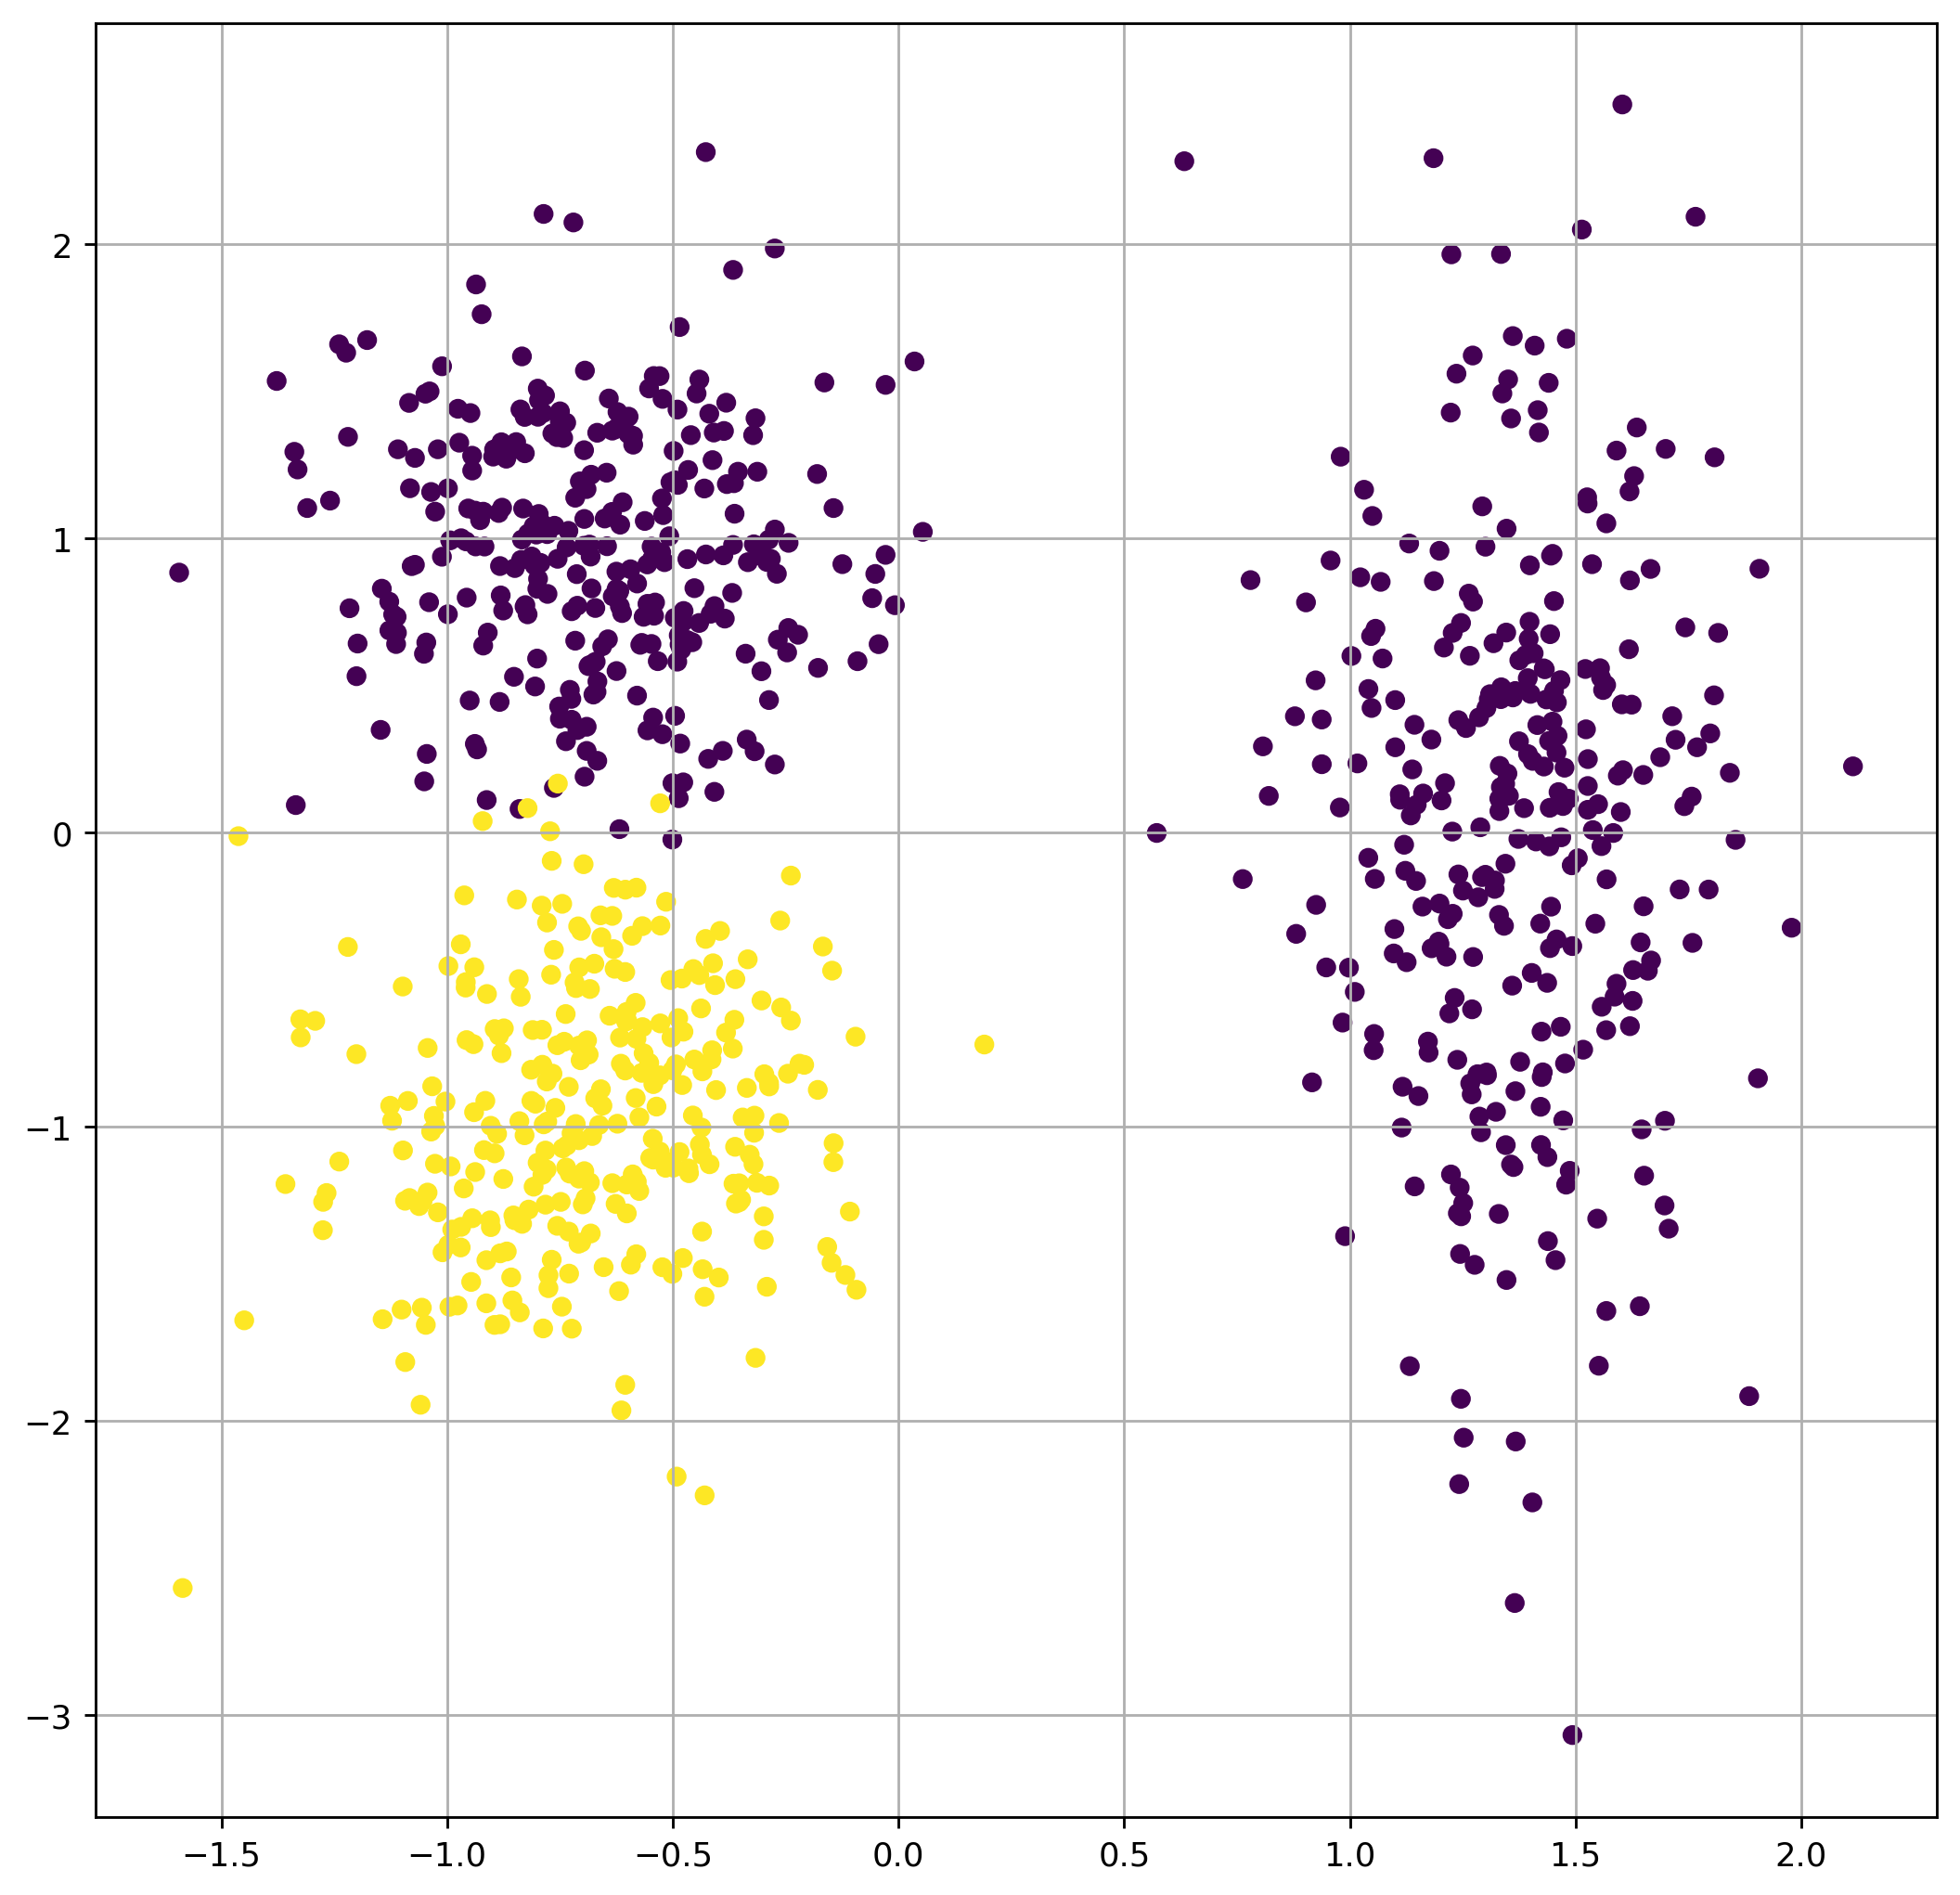
\includegraphics[width=.35\linewidth]{figures/example_groups/groups_centered}}
  ~
  \subfloat[\label{fig:ex-groups-after}]{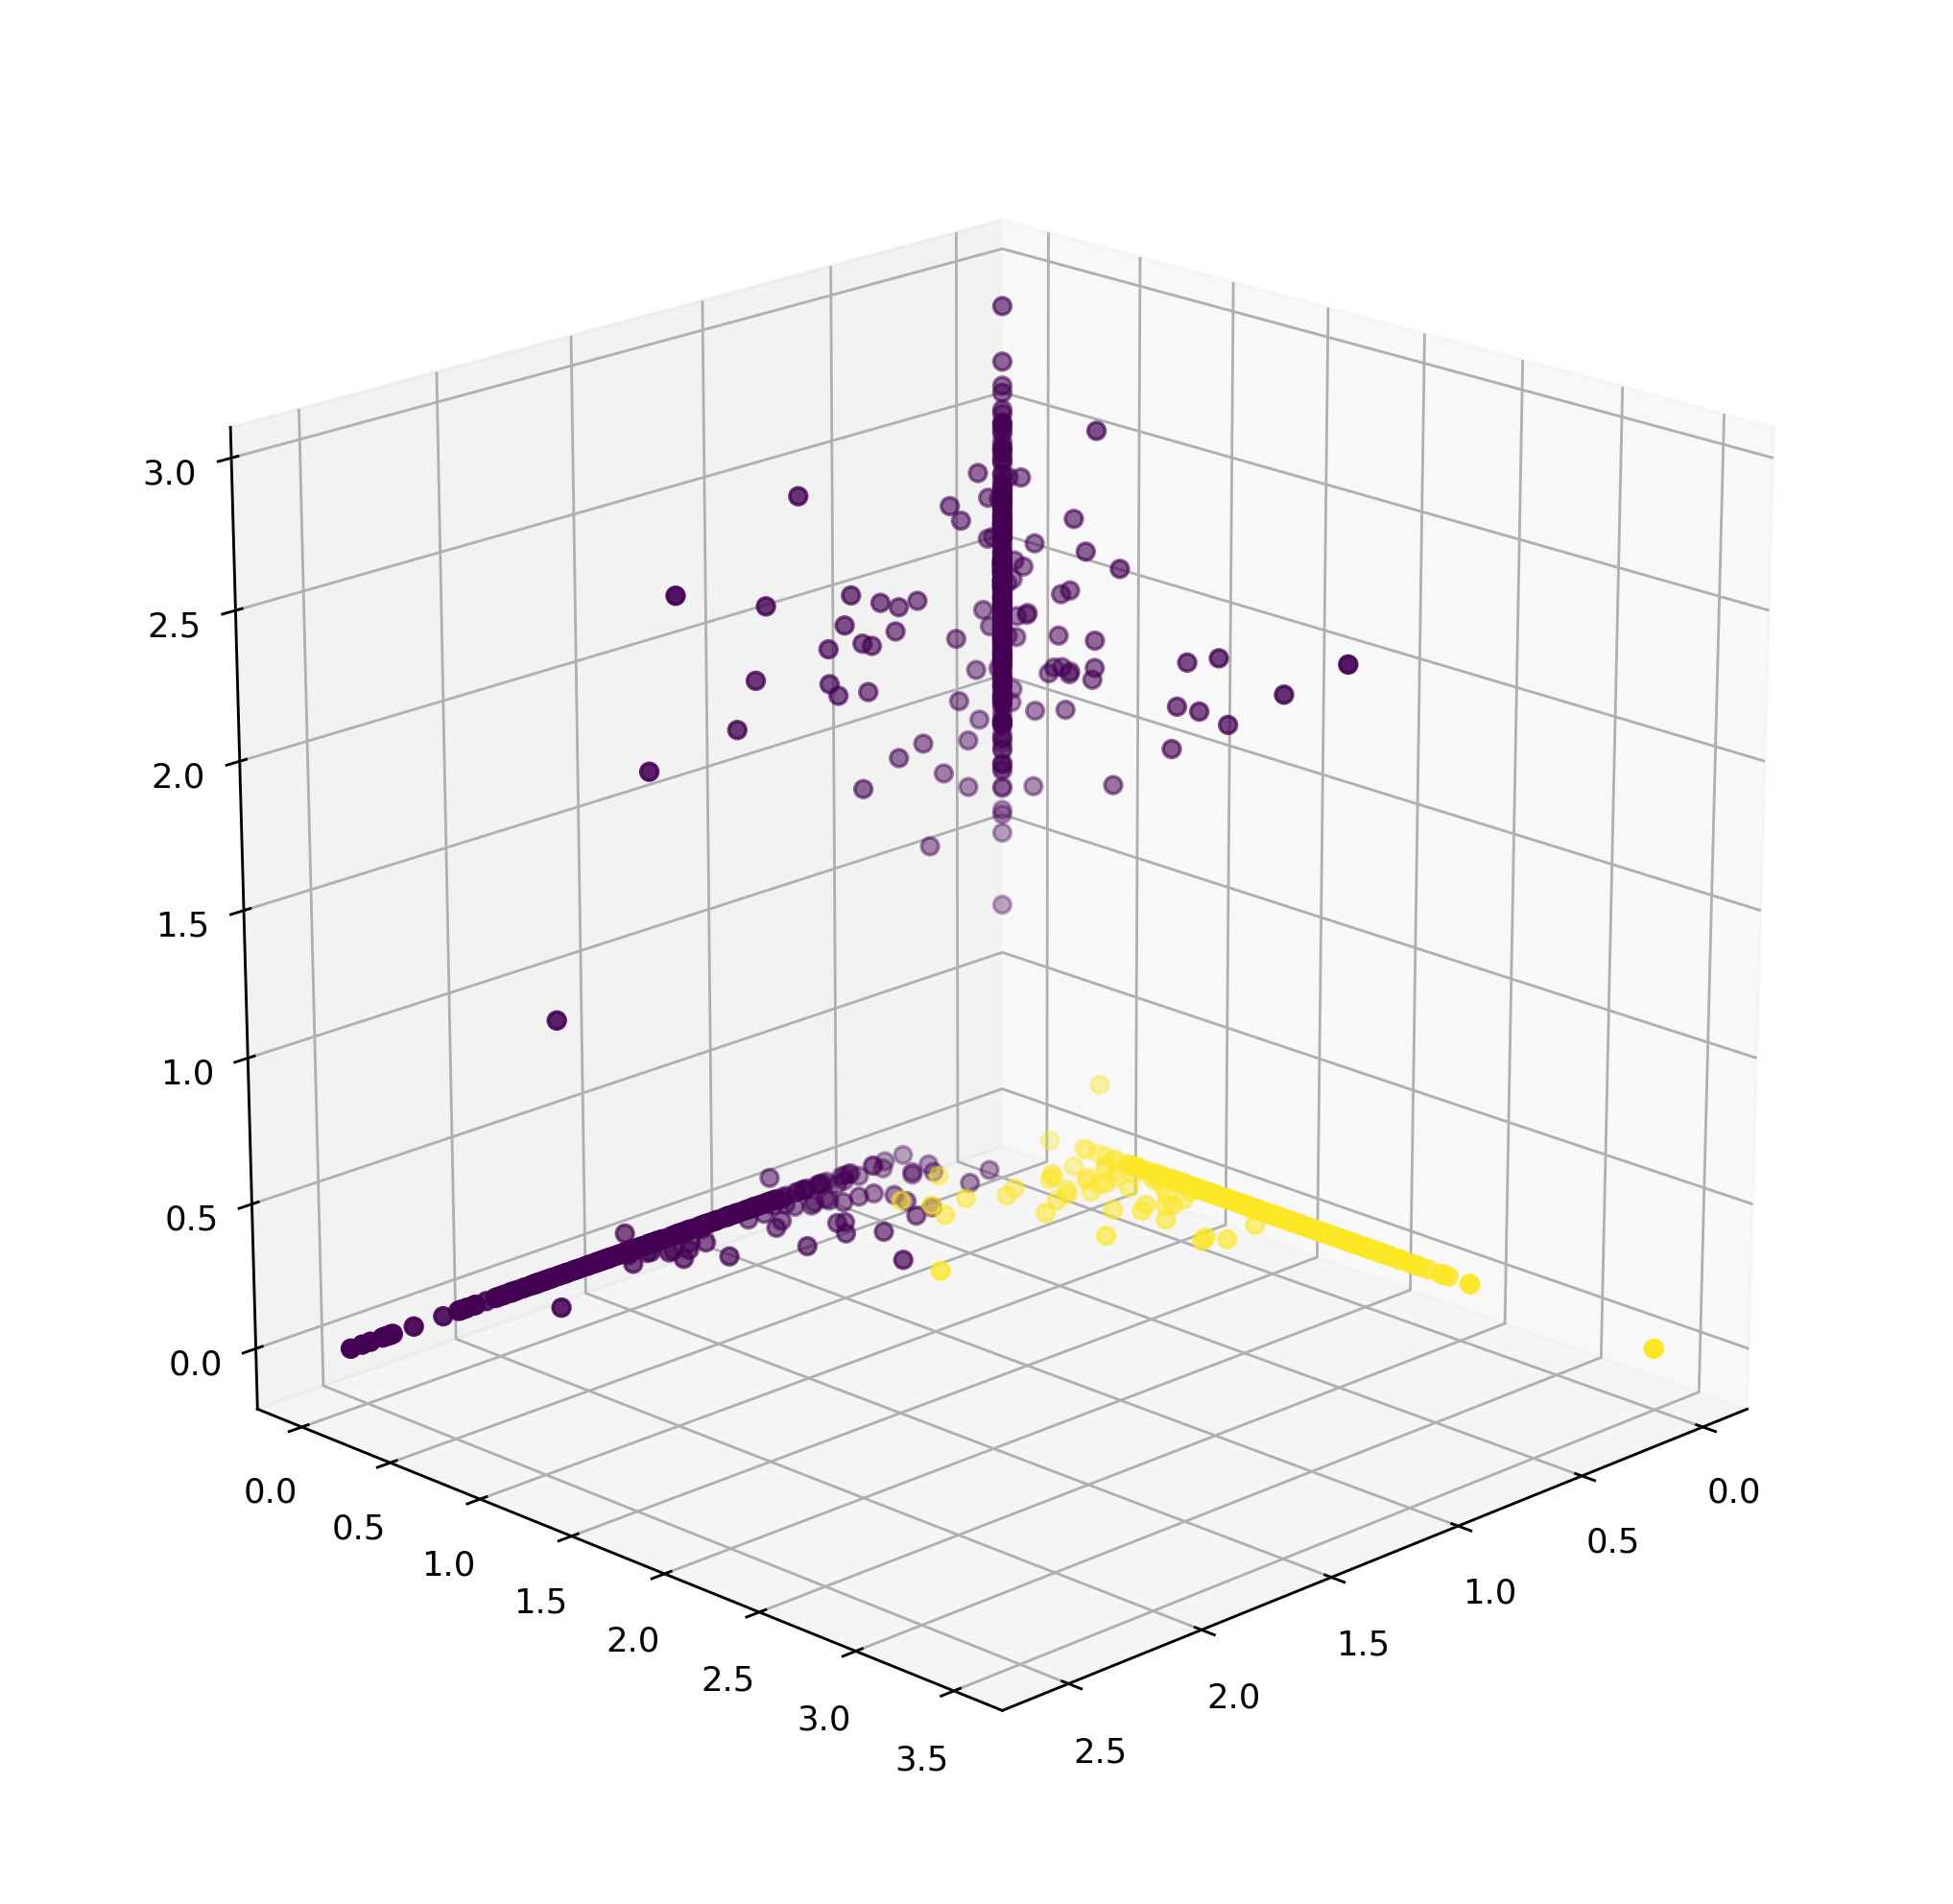
\includegraphics[width=.45\linewidth]{figures/example_groups/groups3d_centered}
  }
  \caption{(a) A 2D feature space with color-coded samples from two classes distributed in three groups. (b) After marker-based batch normalization and convolution with filters obtained from each group, the classes can be more easily detected by two filters in a new 3D feature space.}
  \label{fig:filter}
\end{figure}

Each convolutional layer is trained individually, one layer at a time, to find its filter set ${\cal F}$. The number of filters per layer depends on the clustering technique. We use $K$-means, and then the user must specify the number $K=|{\cal F}|$ of filters. After the convolution operation, we apply the ReLU function to eliminate negative activations and the max-pooling operation to aggregate local information. Note that, apart from the initial marker selection, the training process is automatic. We have preserved the convolutional layers' output dimensions and the marker pixels so we can find the filters of layer $L+1$ from the output of layer $L$. Figure~\ref{fig:arch} shows one example of a simple network projected by FLIM for the experiments of the next section. 

\begin{figure}
  \begin{center}
  \tikzset{
    treenode/.style = {shape=rectangle, rounded corners,
                       draw=black, align=center, line width=width},
    specialedge/.style = {line width=1.5pt}
  }

  \begin{tikzpicture}
    [
      grow                    = down,
      sibling distance        = 5em,
      level distance          = 8mm,
      edge from parent/.style = {draw=black, -latex},
      every node/.style       = {treenode},
      sloped
    ]
    \node [treenode, fill=tealDeer] (v0) {MarkerBased BatchNorm}
    child {
        node [treenode, fill=tealDeer] {Conv$(60 \times 7 \times 7)$}
        child {
          node [treenode, fill=tealDeer] {ReLU} 
          child {
            node [treenode, fill=tealDeer] {MaxPool$(3\times3)$}
            child {
              node [treenode, fill=tealDeer] {BatchNorm}
              child {
                node [treenode, fill=navyPurple] {Classifier}
                edge from parent
              }
            }
          } 
        }
      };

  \end{tikzpicture}
  \end{center}
  \caption{Example of a network with a single convolutional layer followed by a classifier, as projected by FLIM and used for the experiments in this work.}
  \label{fig:arch}
\end{figure}

\section{Experiments}

We used a dataset from~\cite{8899005}, which contains regions of aerial images with and without coconut trees from the Kingdom of Tonga, as acquired in October 2017~\footnote{The images are available in \url{blog.werobotics.org/2018/01/11/open-ai-challenge-2}.}. Each region should be classified as containing one or none coconut tree, but part of coconut trees from adjacent regions might appears near the region's border. The Humanitarian OpenStreetMap community annotated the regions. The dataset consists of 13587 regions with $90 \times 90$ pixels with resolution under $10$\si{\square\centi\metre}, being 10268 and 3319 regions annotated as containing and not containing coconut trees, respectively. The region images are converted to the LAB color space, with each channel normalized within $[0,1]$.

To assess the impact of FLIM in reducing the need for annotated samples, we randomly selected 100 regions from each class for training and left the remaining 11387 regions for testing. We repeated this procedure three times to compute the mean and the standard deviation of the results in precision, recall, and f-score. By vectorizing and projecting the 200 training images of each split on 2D with t-SNE~\cite{maaten2008visualizing}, we identified cohesive groups of images from each class and selected two representative images from each class to draw markers.  The selected images from one split can be seen in Figure \ref{fig:markers}. We placed markers on these images in regions that we thought to better distinguish between coconut and non-coconut classes.

We neither evaluated markers from a higher number of images nor multiple network architectures trained by FLIM. We just trained the single-convolutional-layer network of Figure \ref{fig:arch} from markers drawn in two images per class.
The convolutional layer has $60$ filters with dimension $7 \times 7$ and 3 color channels. It includes marker-based normalization before convolution, ReLu activation, and a max-pooling operation with a window of dimension $3 \times 3$. Since it is the single and last convolutional layer, we applied a stride of $4$ in max-pooling and batch normalization to create an input as close as possible to the one of the MLP classifier used in the popular VGG-16~\cite{simonyan2014very}.

We selected VGG-16 for comparative analysis since it usually requires many more samples than 200 to be trained from scratch. It is also a very competitive CNN when pretrained in the ImageNet dataset, working as an alternative solution for small training sets. Therefore, as baselines, we used three solutions based on VGG-16: (1) VGG is trained from scratch, (2) VGG-FT is pretrained in the ImageNet dataset and fine-tuned in the coconut-tree training set, and (3) VGG-FE is the feature extractor of VGG-16 (the output of the last convolutional layer) pretrained in the ImageNet dataset. In this case, we used for classification the  linear SVM classifier with $C=0.01$ from sklearn~\cite{fan2008liblinear, scikit-learn}.

Table~\ref{tab:results} shows the results of three FLIM-based solutions using the SVM and MLP classifiers; "FLIM + SVM", "FLIM + MLP", and "FLIM-FT + MLP" (i.e., FLIM with fine-tuning); compared with the VGG-based solutions above. The first two rows indicate that FLIM  can provide a more effective feature extractor using a single convolutional layer than VGG-FE, which contains 13 convolutional layers pretrained on the ImageNet. The results of "FLIM + MLP" and "FLIM-FT + MLP" show that FLIM  may dismiss fine tuning by providing a more effective solution. By comparing "FLIM + MLP" with VGG, one can observe that FLIM reduces the number of required training images. Finally, the comparison between "FLIM + MLP" and VGG-FT demonstrates that FLIM can provide competitive results using a considerably more simplified architecture than  VGG-FT. The number of parameters of our feature extractor represents only $0.07\%$ of the number of parameter of VGG16's feature extractor.

\begin{figure}[!t]
    \centering
    \subfloat[\label{fig:markers1}]{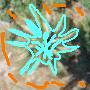
\includegraphics[width=.3\linewidth]{figures/markers1}
    }
    ~
    \subfloat[\label{fig:markers2}]{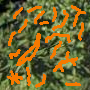
\includegraphics[width=.3\linewidth]{figures/markers2}
    }
    \\
    \subfloat[\label{fig:markers3}]{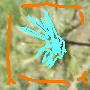
\includegraphics[width=.3\linewidth]{figures/markers3}
    }
    ~
    \subfloat[\label{fig:markers4}]{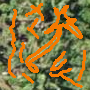
\includegraphics[width=.3\linewidth]{figures/markers4}
    }
    \caption{Markers used for training in image regions with (first column) and without (second column) a coconut tree.}
    \label{fig:markers}
\end{figure}

\begin{table}[!t]
  \begin{center}
  \begin{tabular}{|l|c|c|c|}
  \hline
   Method & Precision & Recall & F-score \\
  \hline\hline
    FLIM + SVM & $0.856 \pm 0.011 $ & $ 0.831 \pm 0.019$ & $ 0.838 \pm 0.017$\\ 
    VGG-FE + SVM & $0.855 \pm 0.001$ & $0.816 \pm 0.007$ & $0.826 \pm 0.006 $ \\\hline
      
    FLIM + MLP & $0.863 \pm 0.002$ & $0.849 \pm 0.005$ & $0.854 \pm 0.004$\\
    FLIM-FT + MLP & $0.845 \pm 0.003$ & $0.825\pm 0.006$ & $0.832 \pm 0.005$ \\

    VGG & $0.827 \pm 0.003$ & $0.770 \pm 0.016$  & $ 0.784 \pm 0.014$\\
    VGG-FT & $0.872 \pm 0.007$ & $0.844 \pm 0.015$ & $0.851 \pm 0.014 $ \\
   
  \hline
  \end{tabular}
  \end{center}

\caption{Mean and standard deviation of precision, recall, and f-score for each method: a feature extractor with a classifier.}
  \label{tab:results}
\end{table}



\begin{figure*}
  \centering
  \subfloat{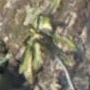
\includegraphics[width=.13\linewidth]{figures/qualitative/ours/upper-coco-108.png}
  }
  ~
  \subfloat{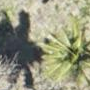
\includegraphics[width=.13\linewidth]{figures/qualitative/ours/upper-coco-2473.png}
  }
  ~
  \subfloat{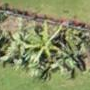
\includegraphics[width=.13\linewidth]{figures/qualitative/ours/upper-non_coco-506.png}
  }
  ~
  \subfloat{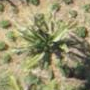
\includegraphics[width=.13\linewidth]{figures/qualitative/vgg/lower-coco-1098.png}
  }
  ~
  \subfloat{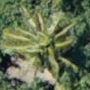
\includegraphics[width=.13\linewidth]{figures/qualitative/vgg/lower-coco-2400.png}
  }
  ~
  \subfloat{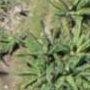
\includegraphics[width=.13\linewidth]{figures/qualitative/vgg/lower-non_coco-105.png}
  }
  \caption{Misclassified images. The first row has images misclassified by the network trained by our method, and the second row has images misclassified by VGG-16. The two first images of a row have coconut trees.}
  \label{fig:ex-classification}
\end{figure*}

 In Figure \ref{fig:ex-classification}, we can see examples of misclassified images. In these images, coconut trees appear in different angles, sizes, and shapes, or the boundaries between the coconut tree and the background are tenuous, making it more difficult to identify them. In turn, images that do not contain coconut trees, contain trees that resemble their shape. The network designer could put markers in those images in other to improve the feature extractor.

\begin{figure}
  \centering
  \subfloat[\label{fig:vis-input}]{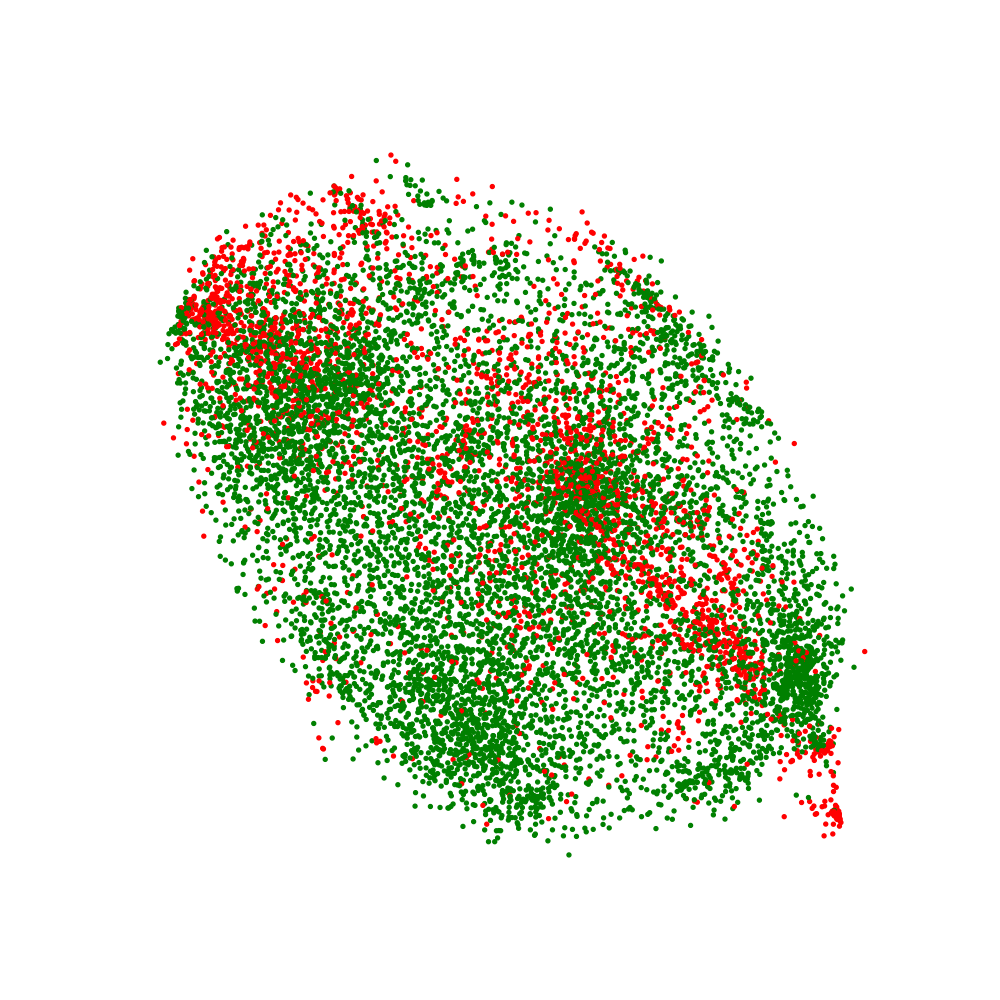
\includegraphics[width=.3\linewidth]{figures/input}
  }
  ~
  \subfloat[\label{fig:vis-feature-extractor}]{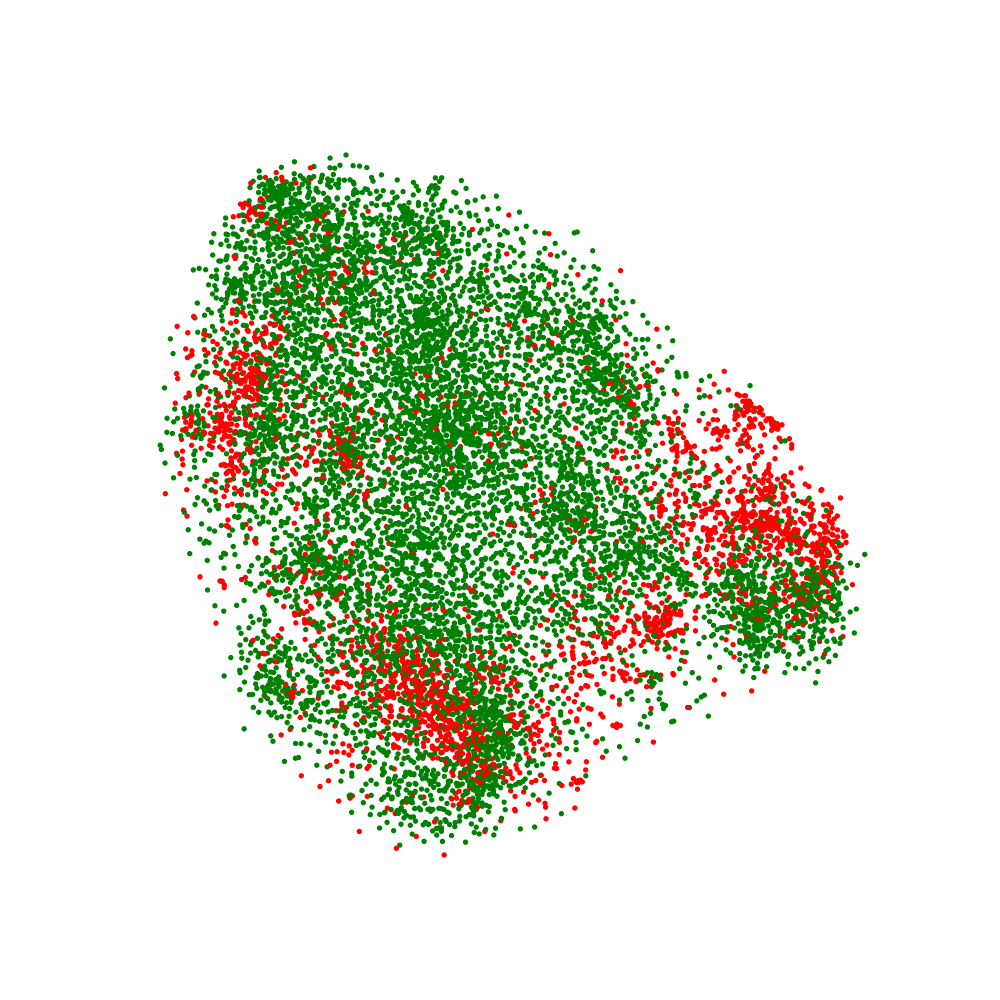
\includegraphics[width=.3\linewidth]{figures/feature_extractor}
  }
  ~
  \subfloat[]{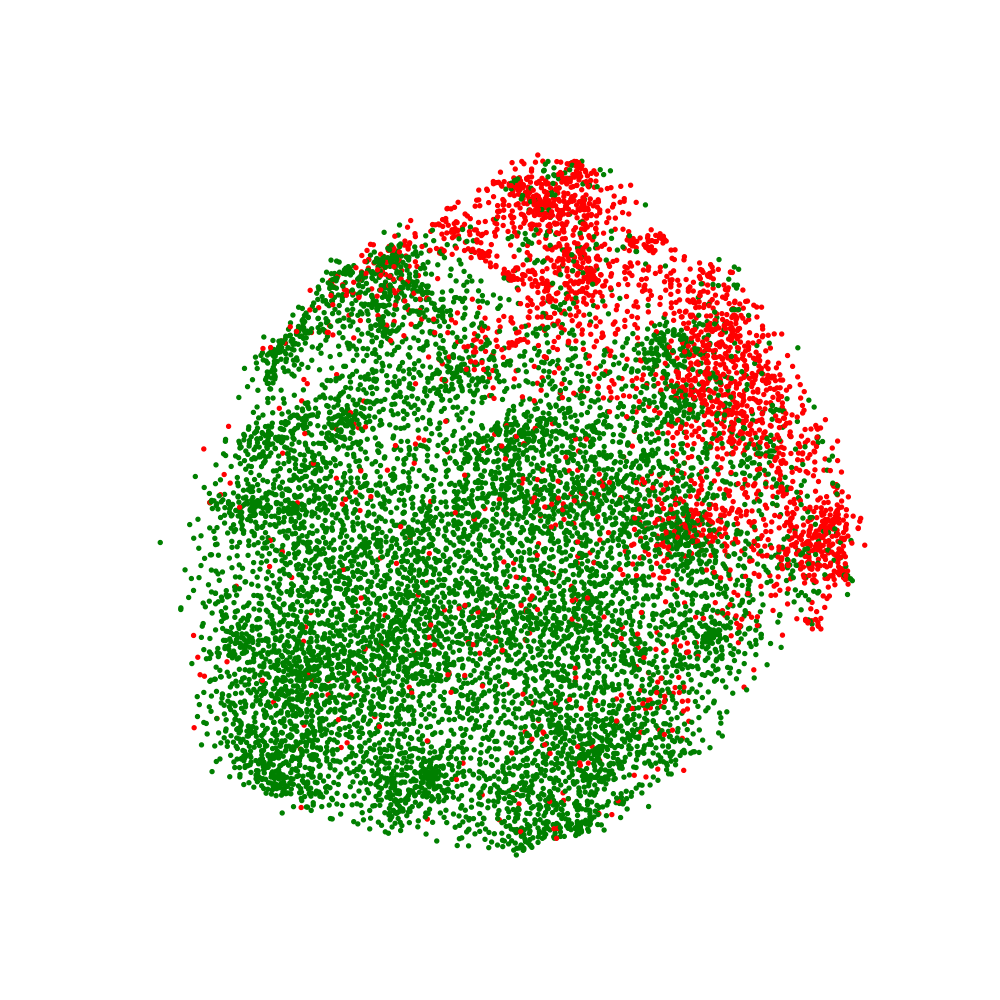
\includegraphics[width=.3\linewidth]{figures/classifier}
  \label{fig:vis-classifier}}
  \caption{Projections by t-SNE of the images at (a) the input layer (original images), (b) the output of the convolutional layer of our network (Figure~\ref{fig:arch}), and (c) the output of the last hidden layer of the MLP classifier in "FLIM + MLP".}
\end{figure}

As motivated by Rauber et al. \cite{rauber2016visualizing}, we made projections of three stages of the network "FLIM + MLP" using t-SNE \cite{maaten2008visualizing} to understand how our CNN transforms the image spaces. In Figure \ref{fig:vis-input}, we can see the projection of the original images (in the LAB color space). Green points are images that contain coconut trees, and red points are images that do not contain coconut trees. The projection shows considerable overlapping between the two classes. Coconut-tree images are more frequent in some regions but they appear very dispersed. In Figure \ref{fig:vis-feature-extractor}, the projection of the output of our feature extractor shows some reduction in the dispersion of the coconut-tree images. The coconut tree images are more concentrated, forming some clusters, and it is possible to notice some overlapping reduction between classes. Finally, Figure \ref{fig:vis-classifier} shows the output of the last hidden layer of the MLP classifier. The overlapping between classes and the dispersion of coconut-tree images are considerably reduced. 

\section{Conclusion}

We introduced a first feature learning technique, named FLIM, that can estimate effective filter weights for the convolutional layers of a given network architecture from user-drawn markers in a few training images. The resulting feature extractor can be used with different classifiers and, when it is used with a MLP classifier, the number of required images to train the fully connected layers is reduced. We demonstrated the advantages of FLIM over solutions based on VGG-16 for binary classification of coconut-tree images. The experiments indicated that FLIM is an effective approach that can produce considerably simplified network architectures. By involving the user in the training process, FLIM improves the understanding about CNN models and the user control over their training process. 

We intend to further investigate feature learning from image markers for different applications, elaborate methodologies to optimize the network architecture, and extend FLIM to estimate weights in fully connected layers.   

\section*{Acknowledgements}

The authors thank FAPESP (Proc. 2014/12236-1), CNPq (Proc. 303808/2018-7), and Unisinos (Viscarb and Visorg projects). 
\bibliographystyle{IEEEtran}
\bibliography{bibliography}

\end{document}


